\begin{figure}[h]
    \centering
    \begin{subfigure}{.3\textwidth}
        \centering
        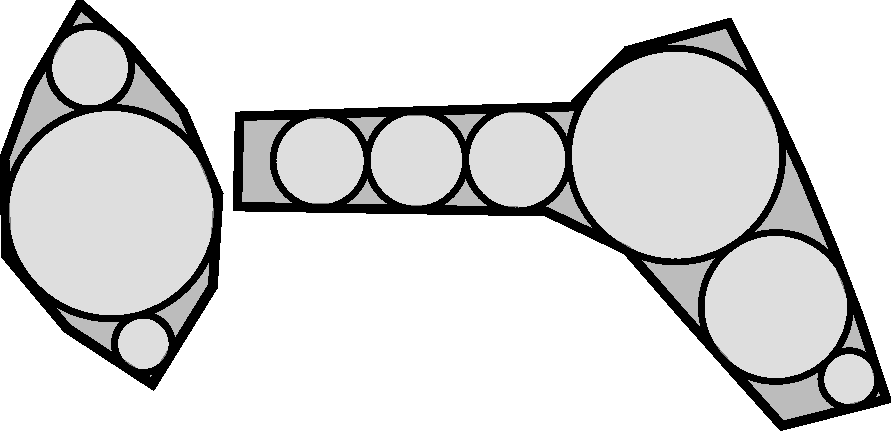
\includegraphics[height=0.4\textwidth]{poles_no_overlap.pdf}
        \caption{Separated}
        \label{fig:poles_no_overlap}
    \end{subfigure}
    \begin{subfigure}{.3\textwidth}
        \centering
        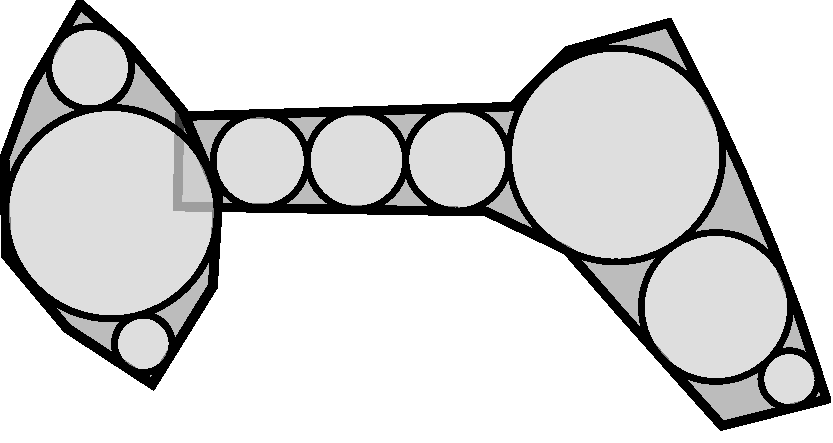
\includegraphics[height=0.4\textwidth]{poles_minor_overlap.pdf}
        \caption{Collision (minor)}
        \label{fig:poles_minor_overlap}
    \end{subfigure}
    \begin{subfigure}{.3\textwidth}
        \centering
        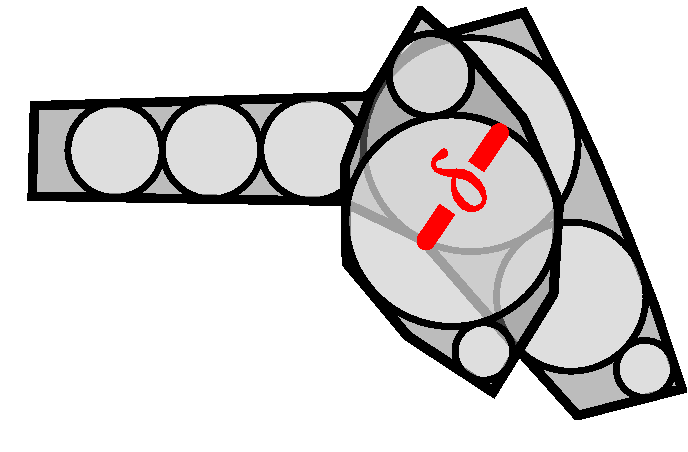
\includegraphics[height=0.4\textwidth]{poles_overlap.pdf}
        \caption{Collision (major)}
        \label{fig:poles_overlap}
    \end{subfigure}
    \caption{Two shapes in different configurations, with their respective poles drawn.
    In (c), the penetration depth ($\delta$) between the largest pair of poles is marked in red.}
    \label{fig:poles}
\end{figure}